\documentclass[a4paper, 11pt]{article}
\usepackage[spanish]{babel}
\usepackage[utf8]{inputenc}
\usepackage{graphicx}
\usepackage{hyperref}
\usepackage{listings}
\usepackage{xcolor}
\usepackage{geometry}
\usepackage{float}
\usepackage{placeins}
\usepackage{caption}
\usepackage{helvet}
\usepackage{setspace}

\geometry{margin=2.5cm}
\renewcommand{\familydefault}{\sfdefault}
\onehalfspacing
\renewcommand{\floatpagefraction}{.8}
\renewcommand{\textfraction}{0.05}   
\renewcommand{\topfraction}{0.8}    
\renewcommand{\bottomfraction}{0.8}
\graphicspath{{images/}}

\title{Plan de Digitalización Integral}
\author{Álvaro Del Valle Fernández}

\begin{document}

\begin{center}
\vspace*{\fill}
{\Huge\textbf{Actividad 6}} \\
\vspace{1cm}
{\LARGE Álvaro Del Valle Fernández}
\vspace*{\fill} 
\end{center}
\newpage

\tableofcontents
\clearpage


\section{Introdución}
    Ahora necesitamos crear el nuevo modulo, para crearlo de forma mas sencilla usaré:\par \bigskip

    \begin{lstlisting}[frame=single,breaklines=true]
    docker exec -it odoo18 odoo scaffold empresaReparto /mnt/extra-addons
    \end{lstlisting}

    \begin{figure}[H]
    \centering
    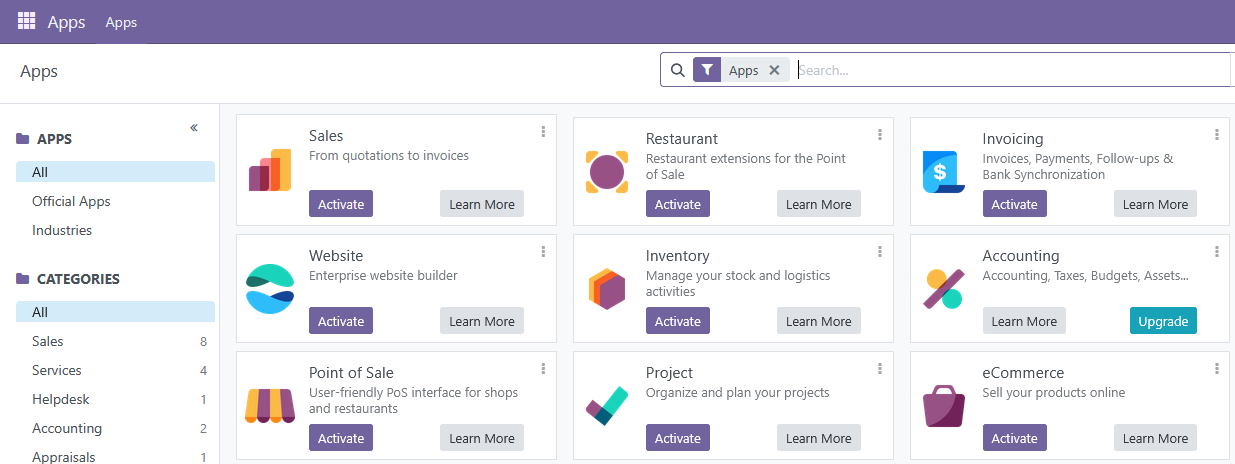
\includegraphics[width=0.8\textwidth]{img2.png}
    \end{figure}



    Ahora creo los modelos que pide el ejercicio:
    \begin{figure}[H]
    \centering
    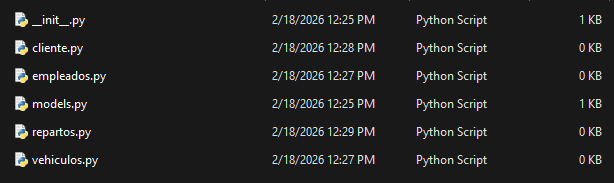
\includegraphics[width=0.8\textwidth]{img5.png}
    \end{figure}


    \begin{lstlisting}[frame=single,breaklines=true]
    cd C:\Users\delva\Desktop\Practica6
    docker compose up --build
    \end{lstlisting}

    Tras multiples horas intenando hacer que funcione odoo creando el modulo desde 0,
    Odoo no es capaz de enviar ningun codigo de error ni indicar por que el modulo se descarga 
    pero no funciona. Debido a esto uso la base del ejericcio 07 de futbol para no perder aun mas tiempo. \par \bigskip

    Tras horas reestructurando el trabajo el modulo nuevo de Futbol adaptado no funciona, al no permitir ni desinstalarlo, no dando error siquiera. \par \bigskip
    Como la version adaptada funcionaba incluso peor decidi volver de nuevo a la primera version, perdiendo todas las horas de trabajo en adaptar la version 07. \par \bigskip

    Esta version no funciona pero por lo menos puedo borrar el modulo y odoo es capaz de indicar algun error aunque nunca de forma precisa.  \par \bigskip
    La base de datos funciona y el modulo se carga, pero los modulos y el wizard dan errores de forma interrumplida, perdiendo horas. \par \bigskip

    \begin{figure}[H]
    \centering
    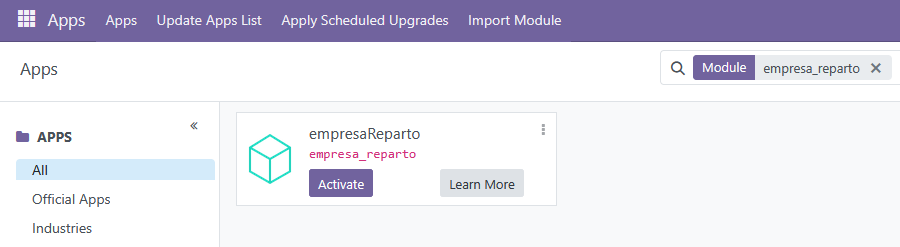
\includegraphics[width=0.8\textwidth]{img6.png}
    \end{figure}


    Tras varias horas de errores entre Odoo y los log de docker consegui la primera version estable:
    \begin{figure}[H]
    \centering
    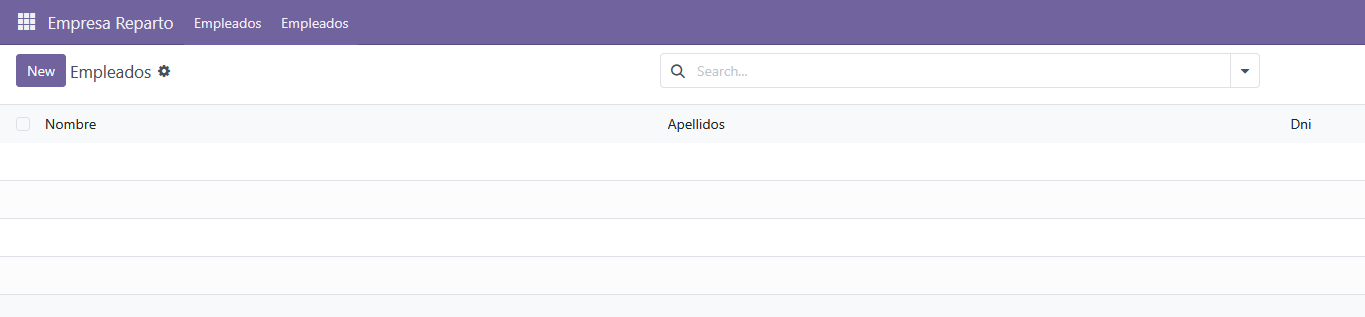
\includegraphics[width=0.8\textwidth]{img7.png}
    \end{figure}

    La version es estable, aunque añadi solo los elemntos basicos junto el primer botón, ahora debo añadir todas las vistas adecuadas.
    \begin{figure}[H]
    \centering
    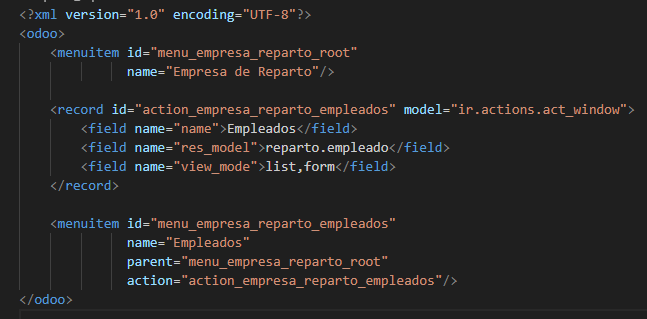
\includegraphics[width=0.8\textwidth]{img8.png}
    \end{figure}
    Elimino el test de boton de empleados dentro de empeladosviews.xml para evitar el duplicado.



\section{Configuración base}
    En este apartado simplemente mostraré los archivos configuración base y de carga de datos.
    \subsection{init.py}
        Indica las rutas de los archivos que deben cargarse:
        \begin{lstlisting}[frame=single,breaklines=true]
        # -*- coding: utf-8 -*-

        from . import models
        from . import controllers 
        from . import wizard
        \end{lstlisting}

    \subsection{manifest.py}
        Elemento de configuracion principal, se encarga de identificar y cargar los elementos,
        simplemente indica dependencias, muestra las rutas de datos a cargar y que se muestre como aplicacion descargable:
        \begin{lstlisting}[frame=single,breaklines=true]
            # -*- coding: utf-8 -*-
            {
                'name': 'Empresa de Repartos',
                'version': '1.0',
                'description': 'Gestion de repartos',
                'author': 'Tu Nombre',
                'depends': ['base'],
                'data': [
                    'security/ir.model.access.csv',
                    'data/sequence_data.xml',
                    'views/empleado_views.xml',
                    'views/vehiculo_views.xml',
                    'views/cliente_views.xml',
                    'views/reparto_views.xml',
                    'views/menu.xml',
                    'reports/reparto_report.xml',
                ],
                'demo': [],
                'installable': True,
                'application': True,
                'license': 'LGPL-3',
            }
        \end{lstlisting}

    \subsection{docker-compose.yml}
        Configuración de docker, configura el contenedor de odoo y el de la base de datos indicando los puertos y rutas.
         Eliminé el campo de version porque daba error.

        \begin{lstlisting}[frame=single,breaklines=true]
            services:
            db:
                image: postgres:15
                container_name: odoo18-db
                environment:
                POSTGRES_DB: postgres
                POSTGRES_USER: odoo
                POSTGRES_PASSWORD: odoo
                volumes:
                - odoo18-db-data:/var/lib/postgresql/data

            odoo:
                image: odoo:18
                container_name: odoo18
                depends_on:
                - db
                ports:
                - "8069:8069"
                volumes:
                - ./addons:/mnt/extra-addons
                - ./config/odoo.conf:/etc/odoo/odoo.conf
                - odoo18-web-data:/var/lib/odoo
                command: odoo -c /etc/odoo/odoo.conf

            volumes:
            odoo18-db-data:
            odoo18-web-data:

        \end{lstlisting}

\section{Models}
Dentro de este apartado mostraré el código de cada uno de los modelos creados, todos siguiendo las indicaciones del ejercicio.
    \subsection{Empleados}
        \begin{lstlisting}[frame=single,breaklines=true]
            from odoo import models, fields, api

            class Empleado(models.Model):
                _name = 'reparto.empleado'
                _description = 'Empleado'

                nombre = fields.Char(required=True)
                apellidos = fields.Char(required=True)
                dni = fields.Char(required=True)
                telefono = fields.Char()
                foto = fields.Binary()
                carnet_ciclomotor = fields.Boolean()
                carnet_furgoneta = fields.Boolean()

                reparto_ids = fields.One2many('reparto.reparto', 'empleado_id')

                def open_repartos_pendientes(self):
                    """Abre el informe de repartos"""
                    self.ensure_one()

                    action = self.env.ref('empresa_reparto.action_report_reparto', raise_if_not_found=False)
                    if not action:

                        return {
                            'type': 'ir.actions.client',
                            'tag': 'display_notification',
                            'params': {
                                'title': 'Error',
                                'message': 'No se encontro la accion del informe',
                                'type': 'danger',
                                'sticky': True,
                            }
                        }
                    return action.report_action(self)
        \end{lstlisting}

    \subsection{Vehículos}
        \begin{lstlisting}[frame=single,breaklines=true]
            from odoo import models, fields, api

            class Vehiculo(models.Model):
                _name = 'reparto.vehiculo'

                tipo = fields.Selection([
                    ('bicicleta', 'Bicicleta'),
                    ('furgoneta', 'Furgoneta')
                ], required=True)

                matricula = fields.Char()
                foto = fields.Binary()
                descripcion = fields.Text()

                estado = fields.Selection([
                    ('disponible', 'Disponible'),
                    ('reparto', 'En reparto')
                ], default='disponible')

        \end{lstlisting}

    \subsection{Clientes}
        \begin{lstlisting}[frame=single,breaklines=true]
            from odoo import models, fields, api

            class Cliente(models.Model):
                _name = 'reparto.cliente'

                dni = fields.Char(required=True)
                nombre = fields.Char(required=True)
                apellidos = fields.Char()
                telefono = fields.Char()
        \end{lstlisting}



        \subsection{Repartos}
        Este es el modelo mas complejo, cumpliendo todas las condiciones del ejercicio. Las restricciones las mostraré en el apartado de restricciones y validaciones, aqui solo muestro el modelo sin restricciones.
        \begin{lstlisting}[frame=single,breaklines=true]
            from odoo import models, fields, api
            from odoo.exceptions import ValidationError

            class Reparto(models.Model):
                _name = 'reparto.reparto'
                _description = 'Reparto'
                _order = 'fecha_recepcion desc, urgencia'

                codigo = fields.Char(default='Nuevo', readonly=True)
                fecha_inicio = fields.Datetime()
                fecha_retorno = fields.Datetime()
                fecha_recepcion = fields.Datetime(required=True)

                empleado_id = fields.Many2one('reparto.empleado', required=True)
                vehiculo_id = fields.Many2one('reparto.vehiculo', required=True)
                kilometros = fields.Float()
                peso = fields.Float()
                volumen = fields.Float()
                observaciones = fields.Text()

                estado = fields.Selection([
                    ('no_salido', 'No ha salido'),
                    ('camino', 'En camino'),
                    ('entregado', 'Entregado')
                ], default='no_salido')

                urgencia = fields.Selection([
                    ('organos', 'Organos humanos'),
                    ('refrigerado', 'Alimentos refrigerados'),
                    ('alimentos', 'Alimentos'),
                    ('alta', 'Alta prioridad'),
                    ('baja', 'Baja prioridad')
                ])

                cliente_id = fields.Many2one('reparto.cliente')
                receptor = fields.Char()
        \end{lstlisting}


\section{Vistas}

    \subsection{Vista menu}
Esta es la vista del menu, simplemente muestra las opciones para cada modelo, indicando el modelo a mostrar y el modo de vista:

        \begin{lstlisting}[frame=single,breaklines=true]
            <?xml version="1.0" encoding="UTF-8"?>
            <odoo>
                <menuitem id="menu_root" name="Empresa de Reparto"/>

                <record id="action_empleados_view" model="ir.actions.act_window">
                    <field name="name">Empleados</field>
                    <field name="res_model">reparto.empleado</field>
                    <field name="view_mode">list,form</field>
                </record>
                <menuitem id="menu_empresa_reparto_empleados"
                        name="Empleados"
                        parent="menu_root"
                        action="action_empleados_view"/>
                <record id="action_vehiculos_view" model="ir.actions.act_window">
                    <field name="name">Vehiculos</field>
                    <field name="res_model">reparto.vehiculo</field>
                    <field name="view_mode">list,form</field>
                </record>
                <menuitem id="menu_empresa_reparto_vehiculos"
                        name="Vehiculos"
                        parent="menu_root"
                        action="action_vehiculos_view"/>

                <record id="action_clientes_view" model="ir.actions.act_window">
                    <field name="name">Clientes</field>
                    <field name="res_model">reparto.cliente</field>
                    <field name="view_mode">list,form</field>
                </record>
                <menuitem id="menu_empresa_reparto_clientes"
                        name="Clientes"
                        parent="menu_root"
                        action="action_clientes_view"/>

                <record id="action_repartos_view" model="ir.actions.act_window">
                    <field name="name">Repartos</field>
                    <field name="res_model">reparto.reparto</field>
                    <field name="view_mode">list,form</field>
                </record>
                <menuitem id="menu_empresa_reparto_repartos"
                        name="Repartos"
                        parent="menu_root"
                        action="action_repartos_view"/>
            </odoo>
        \end{lstlisting}


    \subsection{Vista cliente}
    Aqui se muestra la vista de cliente, con los campos mas importantes, el resto de campos se pueden ver en el formulario:
        \begin{figure}[H]
    \centering
    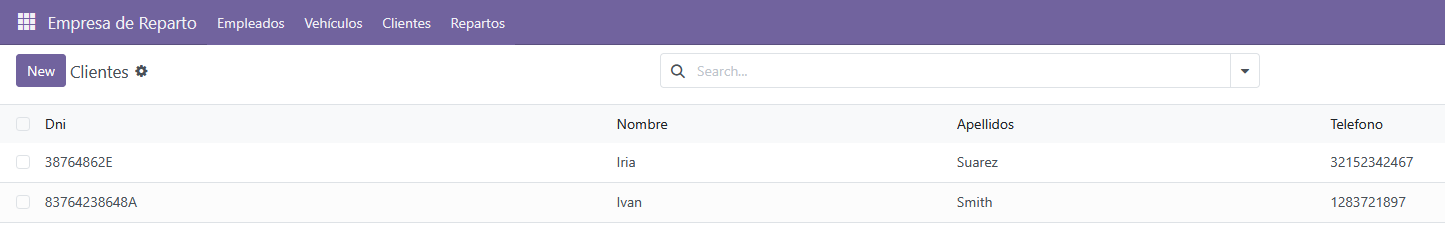
\includegraphics[width=0.8\textwidth]{img22.png}
    \end{figure}
            \begin{figure}[H]
    \centering
    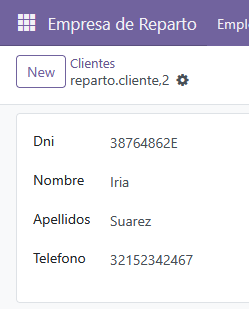
\includegraphics[width=0.8\textwidth]{img26.png}
    \end{figure}
        \begin{lstlisting}[frame=single,breaklines=true]
            <?xml version="1.0" encoding="UTF-8"?>
            <odoo>
                <record id="view_cliente_list" model="ir.ui.view">
                    <field name="name">reparto.cliente.list</field>
                    <field name="model">reparto.cliente</field>
                    <field name="arch" type="xml">
                        <list>
                            <field name="dni"/>
                            <field name="nombre"/>
                            <field name="apellidos"/>
                            <field name="telefono"/>
                        </list>
                    </field>
                </record>

                <record id="view_cliente_form" model="ir.ui.view">
                    <field name="name">reparto.cliente.form</field>
                    <field name="model">reparto.cliente</field>
                    <field name="arch" type="xml">
                        <form>
                            <sheet>
                                <group>
                                    <field name="dni"/>
                                    <field name="nombre"/>
                                    <field name="apellidos"/>
                                    <field name="telefono"/>
                                </group>
                            </sheet>
                        </form>
                    </field>
                </record>
            </odoo>
        \end{lstlisting}
    \subsection{Vista empleado}
    En esta vista podemos ver la informacion mas importante de cada empleado.
    \begin{figure}[H]
    \centering
    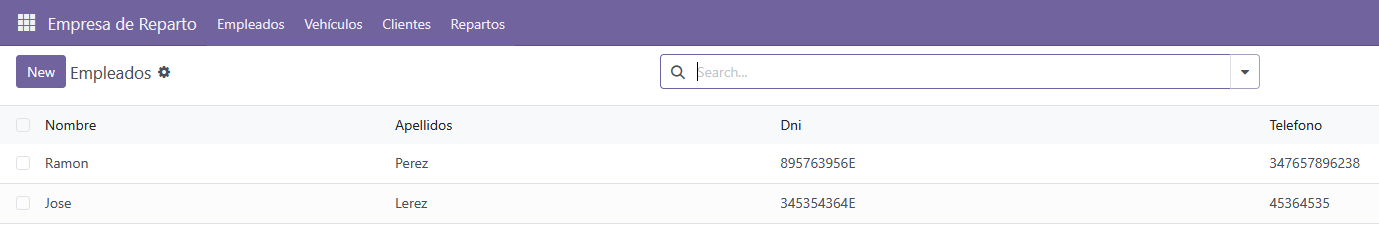
\includegraphics[width=0.8\textwidth]{img21.png}
    \end{figure}
        \begin{figure}[H]
    \centering
    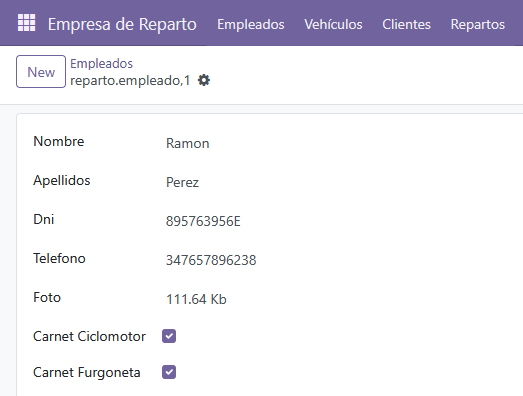
\includegraphics[width=0.8\textwidth]{img25.png}
    \end{figure}
            \begin{figure}[H]
    \centering
    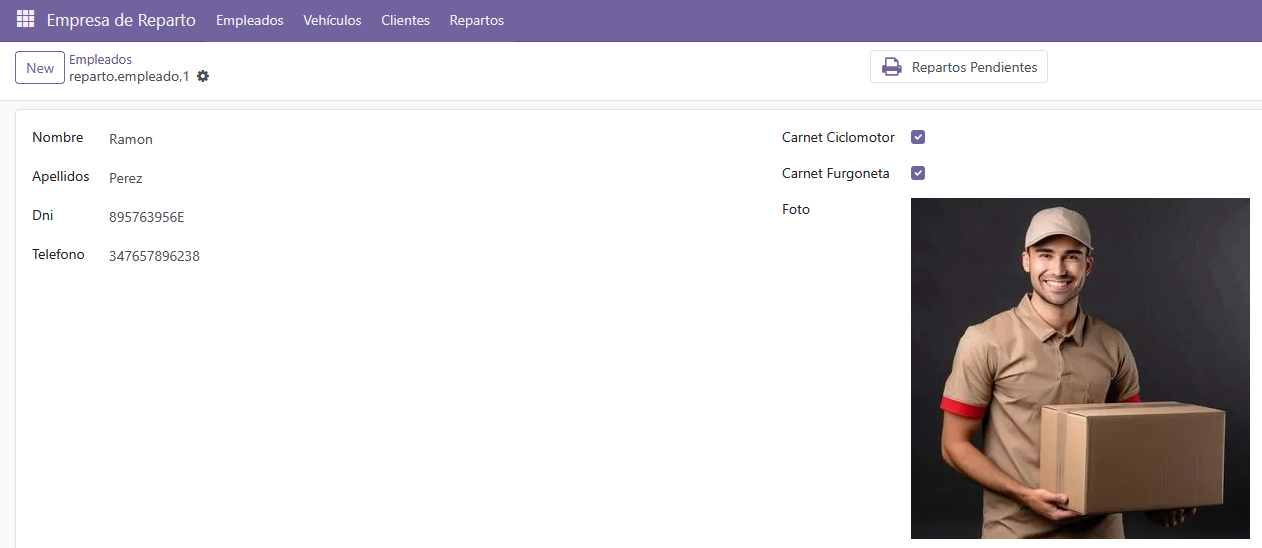
\includegraphics[width=0.8\textwidth]{img17.png}
    \end{figure}
        \begin{lstlisting}[frame=single,breaklines=true]
            <?xml version="1.0" encoding="UTF-8"?>
            <odoo>

                <!-- Vista lista -->
                <record id="view_empleado_list" model="ir.ui.view">
                    <field name="name">empleado.list</field>
                    <field name="model">reparto.empleado</field>
                    <field name="arch" type="xml">
                        <list>
                            <field name="nombre"/>
                            <field name="apellidos"/>
                            <field name="dni"/>
                            <field name="telefono"/>
                        </list>
                    </field>
                </record>

                <!-- Vista formulario -->
                <record id="view_empleado_form" model="ir.ui.view">
                    <field name="name">empleado.form</field>
                    <field name="model">reparto.empleado</field>
                    <field name="arch" type="xml">
                        <form string="Empleado">
                            <sheet>
                                <group>
                                    <field name="nombre"/>
                                    <field name="apellidos"/>
                                    <field name="dni"/>
                                    <field name="telefono"/>
                                    <field name="foto"/>
                                    <field name="carnet_ciclomotor"/>
                                    <field name="carnet_furgoneta"/>
                                </group>
                            </sheet>
                        </form>
                    </field>
                </record>
            </odoo>
        \end{lstlisting}

    \subsection{Vista vehiculo}
    Similar a las vistas anteriores, en esta vista se muestra la informacion mas importante de cada vehiculo.
    \begin{figure}[H]
    \centering
    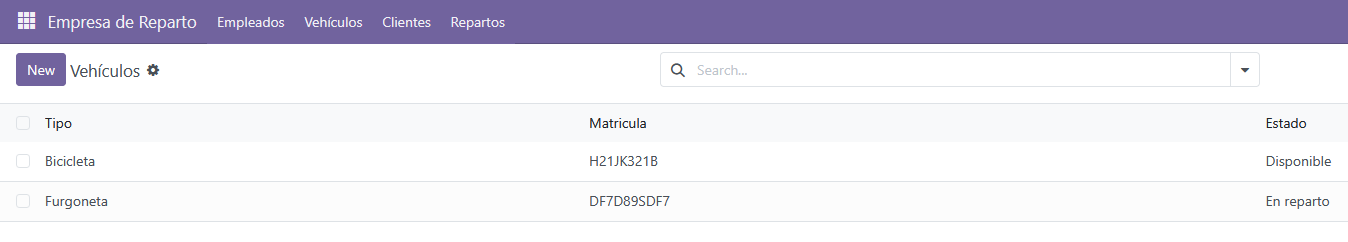
\includegraphics[width=0.8\textwidth]{img23.png}
    \end{figure}
       \begin{figure}[H]
    \centering
    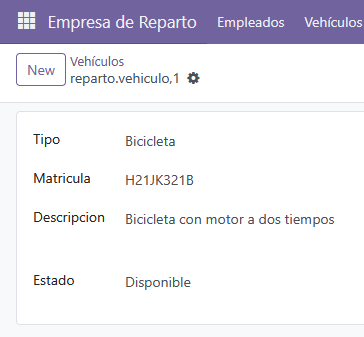
\includegraphics[width=0.8\textwidth]{img27.png}
    \end{figure}
        \begin{lstlisting}[frame=single,breaklines=true]
            <?xml version="1.0" encoding="UTF-8"?>
            <odoo>
                <record id="view_vehiculo_list" model="ir.ui.view">
                    <field name="name">reparto.vehiculo.list</field>
                    <field name="model">reparto.vehiculo</field>
                    <field name="arch" type="xml">
                        <list>
                            <field name="tipo"/>
                            <field name="matricula"/>
                            <field name="estado"/>
                        </list>
                    </field>
                </record>

                <record id="view_vehiculo_form" model="ir.ui.view">
                    <field name="name">reparto.vehiculo.form</field>
                    <field name="model">reparto.vehiculo</field>
                    <field name="arch" type="xml">
                        <form>
                            <sheet>
                                <group>
                                    <field name="tipo"/>
                                    <field name="matricula"/>
                                    <field name="descripcion"/>
                                    <field name="estado"/>
                                </group>
                            </sheet>
                        </form>
                    </field>
                </record>
            </odoo>
        \end{lstlisting}


    \subsection{Vista reparto}
Al utilizar el wizard para crear los repartos, la vista de lista y formulario de reparto es muy simple, mostrando solo los campos basicos, el resto de campos se rellenan en el wizard.
Dentro del apartado de wizard mostraré esa vista de formulario.
    \begin{figure}[H]
    \centering
    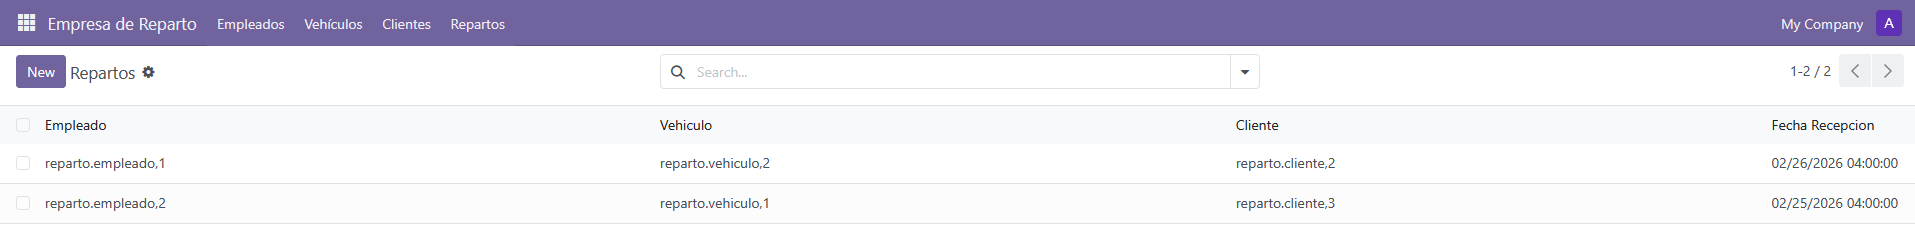
\includegraphics[width=0.8\textwidth]{img24.png}
    \end{figure}
        \begin{figure}[H]
    \centering
    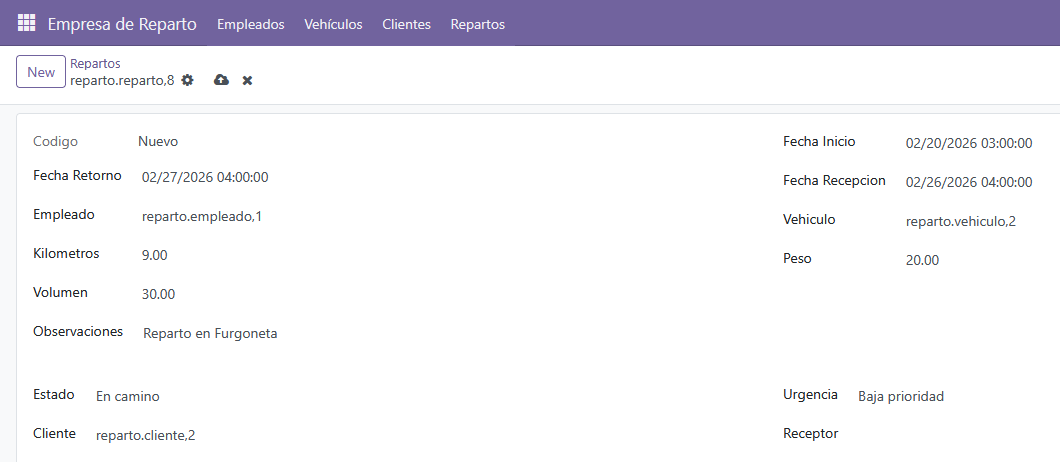
\includegraphics[width=0.8\textwidth]{img28.png}
    \end{figure}
        \begin{lstlisting}[frame=single,breaklines=true]
            <?xml version="1.0" encoding="UTF-8"?>
            <odoo>
                <record id="view_reparto_list" model="ir.ui.view">
                    <field name="name">reparto.list</field>
                    <field name="model">reparto.reparto</field>
                    <field name="arch" type="xml">
                        <list>
                            <field name="empleado_id"/>
                            <field name="vehiculo_id"/>
                            <field name="cliente_id"/>
                            <field name="fecha_recepcion"/>
                        </list>
                    </field>
                </record>

                <record id="action_repartos_view" model="ir.actions.act_window">
                    <field name="name">Repartos</field>
                    <field name="res_model">reparto.reparto</field>
                    <field name="view_mode">list,form</field>
                    <field name="context">{'default_open_wizard': True}</field>
                </record>
            </odoo>
        \end{lstlisting}



\section{Restricciones y validaciones}
Ahora mostraré mas restricciones pedidas en el enunciado
    \subsection{Empleado no tiene el carnet}
Codigo para validar:
    \begin{lstlisting}[frame=single,breaklines=true]
            @api.constrains('empleado_id', 'vehiculo_id')
    def _check_carnet(self):
        for record in self:
            if record.vehiculo_id.tipo == 'bicicleta' and not record.empleado_id.carnet_ciclomotor:
                raise ValidationError("El empleado no tiene carnet de ciclomotor.")
            if record.vehiculo_id.tipo == 'furgoneta' and not record.empleado_id.carnet_furgoneta:
                raise ValidationError("El empleado no tiene carnet de furgoneta.")
        \end{lstlisting}  

    \subsection{Si el empleado o vehiculo ya estan en otro reparto:}
    \begin{lstlisting}[frame=single,breaklines=true]
        @api.constrains('empleado_id', 'estado')
        def _check_reparto_activo(self):
            for record in self:
                activos = self.search([
                    ('empleado_id', '=', record.empleado_id.id),
                    ('estado', '=', 'camino'),
                    ('id', '!=', record.id)
                ])
                if activos and record.estado == 'camino':
                    raise ValidationError("El empleado ya tiene un reparto activo.")
               \end{lstlisting}

    \subsection{Repartos de mas de 10km no se pueden realizar en bicicleta:}
    Codigo para validar:
    \begin{lstlisting}[frame=single,breaklines=true]
    @api.constrains('kilometros', 'vehiculo_id')
    def _check_km(self):
        for record in self:
            if record.vehiculo_id.tipo == 'bicicleta' and record.kilometros > 10:
                raise ValidationError("Mas de 10km no puede hacerse en bicicleta.")
            
             \end{lstlisting}
    \subsection{Repartos de menos de 1km no se pueden realizar en furgoneta:}
    \begin{lstlisting}[frame=single,breaklines=true]
            if record.vehiculo_id.tipo == 'furgoneta' and record.kilometros < 1:
                raise ValidationError("Menos de 1km no puede hacerse en furgoneta.")
             \end{lstlisting}


    \subsection{Repartos ordenados por fecha de recepcion y urgencia:}
    Simplemente con el campo order los repartos se ordenan correctamente:
    \begin{lstlisting}[frame=single,breaklines=true]
        _order = 'fecha_recepcion desc, urgencia'
    \end{lstlisting}
    \subsection{Colores diferentes segun el estado del reparto:}
    El atributo decoración cambia el color del texto segun el estado:
    \begin{lstlisting}[frame=single,breaklines=true]
        <list
            decoration-danger="estado == 'camino'"
            decoration-success="estado == 'entregado'"
            decoration-muted="estado == 'no_salido'">
    \end{lstlisting}
\begin{figure}[H]
    \centering
    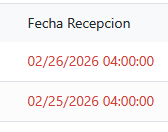
\includegraphics[width=0.8\textwidth]{img29.png}
    \end{figure}


\section{Wizard}
    Wizard para repartos, al hacer click en New se abre el wizard para rellenar los campos necesarios, ahora msotraré los documentos.
    Tambien realiza un check por si no cumple las restricciones definidas en el modelo reparto. \\
    Primero el reparto wizard py:
    \begin{lstlisting}[frame=single,breaklines=true]
        from odoo import models, fields, api
        from odoo.exceptions import ValidationError

        class RepartoWizard(models.TransientModel):
            _name = 'reparto.reparto_wizard'

            empleado_id = fields.Many2one('reparto.empleado', string="Empleado", required=True)
            vehiculo_id = fields.Many2one('reparto.vehiculo', string="Vehiculo", required=True)
            cliente_id = fields.Many2one('reparto.cliente', string="Cliente", required=True)
            def crear_reparto(self):
                Reparto = self.env['reparto.reparto']

        #Crear el reparto
                reparto = Reparto.new({
                    'empleado_id': self.empleado_id.id,
                    'vehiculo_id': self.vehiculo_id.id,
                    'cliente_id': self.cliente_id.id,
                    'fecha_recepcion': fields.Datetime.now(),
                    'estado': 'camino',
                })

                reparto._check_carnet()
                reparto._check_reparto_activo()
                reparto._check_km()
                reparto_id = Reparto.create(reparto._convert_to_write(reparto._cache))
                return {'type': 'ir.actions.act_window_close'}
    \end{lstlisting}



Ahora el reparto wizard xml que se encarga de la estructura de la vista del wizard:
    \begin{lstlisting}[frame=single,breaklines=true]
        <!--Vista-->
            <record id="view_reparto_wizard_form" model="ir.ui.view">
                <field name="name">reparto.wizard.form</field>
                <field name="model">reparto.reparto_wizard</field>
                <field name="arch" type="xml">
                    <form string="Crear Reparto">
                        <group>
                            <field name="empleado_id"/>
                            <field name="vehiculo_id"/>
                            <field name="cliente_id"/>
                        </group>
                        <footer>
                            <button string="Crear" type="object" name="crear_reparto" class="btn-primary"/>
                            <button string="Cancelar" class="btn-secondary" special="cancel"/>
                        </footer>
                    </form>
                </field>
            </record>
        <!--Abrir -->
            <record id="action_reparto_wizard" model="ir.actions.act_window">
                <field name="name">Crear Reparto</field>
                <field name="res_model">reparto.reparto_wizard</field>
                <field name="view_mode">form</field>
                <field name="target">new</field>
            </record>
        </odoo>
    \end{lstlisting}



\section{Informes}
    Informe para cada empleado con los repartos pendientes, este elemento se situa en reports, reparto report. xml y es activado
     mediante el boton de la vista de empleado, el cual abre el informe. \\
    \begin{lstlisting}[frame=single,breaklines=true]
        <?xml version="1.0" encoding="utf-8"?>
        <odoo>
            <template id="report_repartos_pendientes_empleado">
                <t t-call="web.html_container">
                    <t t-foreach="docs" t-as="empleado">
                        <t t-call="web.external_layout">
                            <div class="page">
                                <div class="oe_structure"/>
                                <div class="row">
                                    <div class="col-xs-12">
                                        <h2>Repartos Pendientes - <t t-esc="empleado.nombre"/> <t t-esc="empleado.apellidos"/></h2>
                                        <p><strong>DNI:</strong> <t t-esc="empleado.dni"/></p>
                                    </div>
                                </div>
                                <div class="row">
                                    <div class="col-xs-12">
                                        <table class="table table-bordered">
                                            <thead>
                                                <tr>
                                                    <th>Codigo</th>
                                                    <th>Cliente</th>
                                                    <th>Vehiculo</th>
                                                    <th>Fecha recepcion</th>
                                                    <th>Urgencia</th>
                                                </tr>
                                            </thead>
                                            <tbody>
                                                <t t-set="repartos_pendientes" t-value="empleado.reparto_ids.filtered(lambda r: r.estado == 'no_salido')"/>
                                                <t t-foreach="repartos_pendientes" t-as="r">
                                                    <tr>
                                                        <td><t t-esc="r.codigo"/></td>
                                                        <td><t t-esc="r.cliente_id.nombre or ''"/> <t t-esc="r.cliente_id.apellidos or ''"/></td>
                                                        <td><t t-esc="r.vehiculo_id.tipo or ''"/></td>
                                                        <td><t t-esc="r.fecha_recepcion"/></td>
                                                        <td><t t-esc="r.urgencia"/></td>
                                                    </tr>
                                                </t>
                                                <t t-if="not repartos_pendientes">
                                                    <tr>
                                                        <td colspan="5" style="text-align: center;">No hay repartos pendientes</td>
                                                    </tr>
                                                </t>
                                            </tbody>
                                        </table>
                                    </div>
                                </div>
                            </div>
                        </t>
                    </t>
                </t>
            </template>

            <record id="action_report_reparto" model="ir.actions.report">
                <field name="name">Repartos pendientes</field>
                <field name="model">reparto.empleado</field>
                <field name="report_type">qweb-pdf</field>
                <field name="report_name">empresa_reparto.report_repartos_pendientes_empleado</field>
                <field name="report_file">empresa_reparto.report_repartos_pendientes_empleado</field>
                <field name="binding_model_id" ref="model_reparto_empleado"/>
                <field name="binding_type">report</field>
                <field name="print_report_name">'Repartos_Pendientes_%s' % (object.nombre)</field>
            </record>
        </odoo>
    \end{lstlisting}
Archivo Reparto. py:
    \begin{lstlisting}[frame=single,breaklines=true]
        from odoo import models

        class ReportRepartoPendientes(models.AbstractModel):
            _name = 'report.empresa_reparto.report_repartos_pendientes_empleado'
            _description = 'Reporte de Repartos Pendientes'

            def _get_report_values(self, docids, data=None):
                docs = self.env['reparto.empleado'].browse(docids)
                return {
                    'doc_ids': docids,
                    'doc_model': 'reparto.empleado',
                    'docs': docs,
                }
    \end{lstlisting}

    Aqui podemos ver un reporte creado correctamente:
\begin{figure}[H]
    \centering
    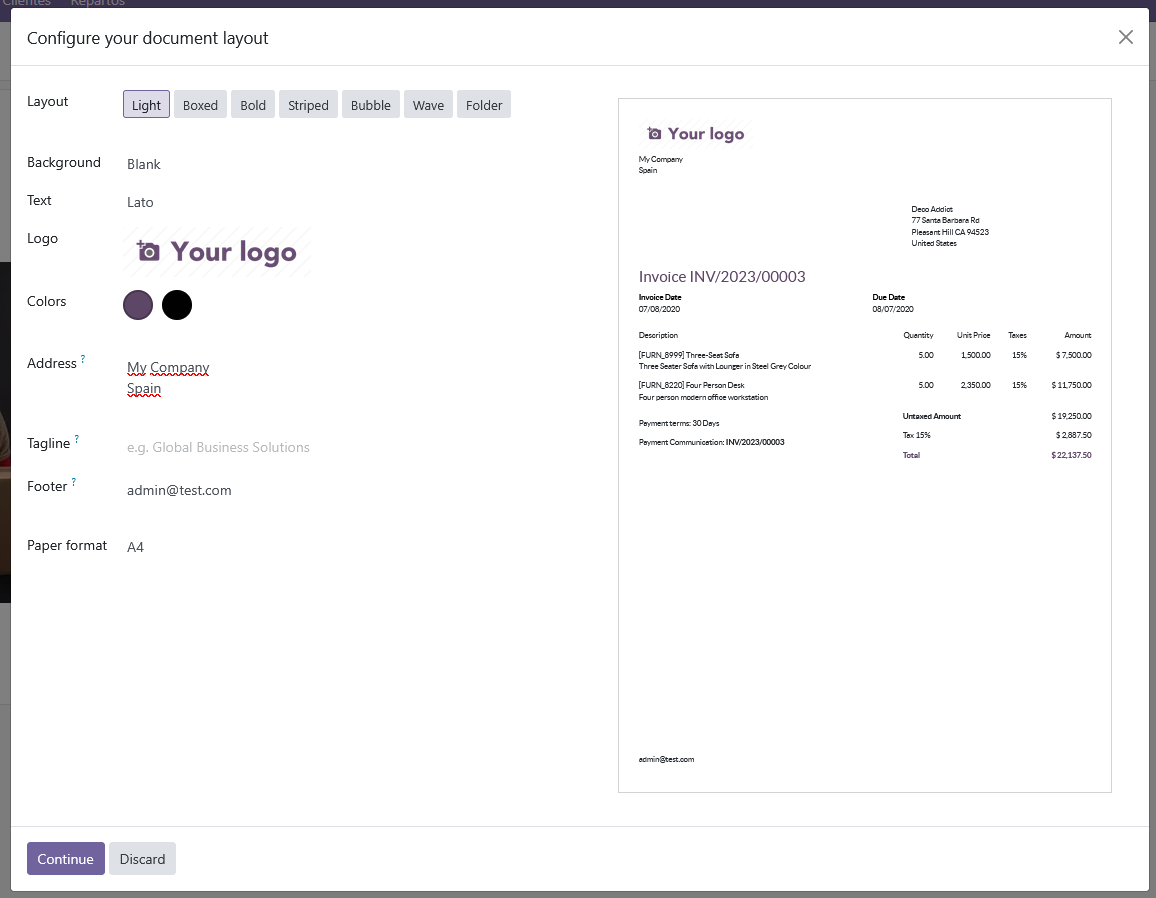
\includegraphics[width=0.8\textwidth]{img30.png}
    \end{figure}
\begin{figure}[H]
    \centering
    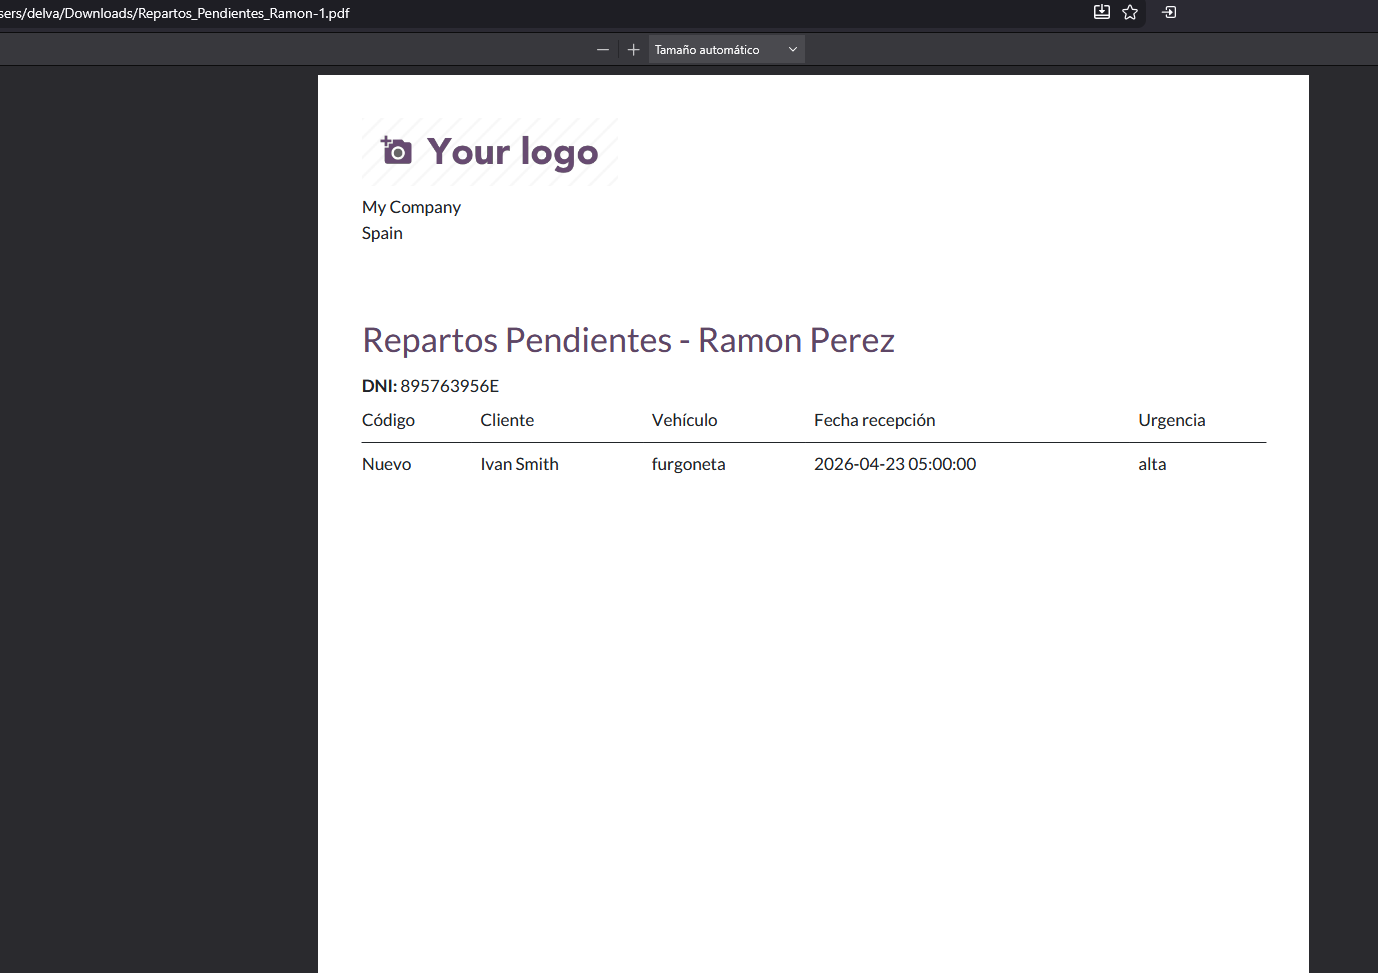
\includegraphics[width=0.8\textwidth]{img33.png}
    \end{figure}

\section{Controlador web}
    Controlador web, esta es la version estable del controlador, no encontré una forma de que no me diese error con la id del reparto.
    Esta se compone de tres endpoints, endpoint que obtiene un JSON mediante el codigo, endpoint JSON listado y el endpoint para 
    el html el cual permite mostrar la interfaz:
    \begin{lstlisting}[frame=single,breaklines=true]
        from odoo import http
from odoo.http import request
import json

class RepartoController(http.Controller):

    @http.route('/repartos/estado/<string:codigo_reparto>', type='http', auth='public', methods=['GET'], csrf=False)
    def obtener_estado_reparto(self, codigo_reparto, **kwargs):
        try:
            reparto = request.env['reparto.reparto'].sudo().search([
                ('codigo', '=', codigo_reparto)
            ], limit=1)
#test error de id
            if not reparto and codigo_reparto.isdigit():
                reparto = request.env['reparto.reparto'].sudo().browse(int(codigo_reparto))
            
            if not reparto:
                return request.make_response(
                    json.dumps({
                        'success': False,
                        'error': f'No se encontro el reparto con codigo: {codigo_reparto}'
                    }, ensure_ascii=False),
                    headers=[('Content-Type', 'application/json')]
                )
            
#Obtener la info 
            estado_texto = dict(reparto._fields['estado'].selection).get(reparto.estado)
            urgencia_texto = dict(reparto._fields['urgencia'].selection).get(reparto.urgencia)
            
            resultado = {
                'success': True,
                'data': {
                    'codigo': reparto.codigo,
                    'id': reparto.id,
                    'estado': reparto.estado,
                    'estado_descripcion': estado_texto,
                    'urgencia': reparto.urgencia,
                    'urgencia_descripcion': urgencia_texto,
                    'fecha_recepcion': reparto.fecha_recepcion.strftime('%d/%m/%Y %H:%M') if reparto.fecha_recepcion else None,
                    'fecha_inicio': reparto.fecha_inicio.strftime('%d/%m/%Y %H:%M') if reparto.fecha_inicio else None,
                    'fecha_retorno': reparto.fecha_retorno.strftime('%d/%m/%Y %H:%M') if reparto.fecha_retorno else None,
                    'repartidor': {
                        'id': reparto.empleado_id.id,
                        'nombre': reparto.empleado_id.nombre,
                        'apellidos': reparto.empleado_id.apellidos,
                        'dni': reparto.empleado_id.dni
                    } if reparto.empleado_id else None,
                    'vehiculo': {
                        'id': reparto.vehiculo_id.id,
                        'tipo': reparto.vehiculo_id.tipo,
                        'descripcion': reparto.vehiculo_id.descripcion,
                        'matricula': reparto.vehiculo_id.matricula
                    } if reparto.vehiculo_id else None,
                    'cliente_emisor': {
                        'id': reparto.cliente_id.id,
                        'nombre': reparto.cliente_id.nombre,
                        'apellidos': reparto.cliente_id.apellidos,
                        'dni': reparto.cliente_id.dni
                    } if reparto.cliente_id else None,
                    'receptor': reparto.receptor,
                    'kilometros': reparto.kilometros,
                    'peso': reparto.peso,
                    'volumen': reparto.volumen,
                    'observaciones': reparto.observaciones
                }
            }
            
            return request.make_response(
                json.dumps(resultado, ensure_ascii=False),
                headers=[('Content-Type', 'application/json')]
            )
            
        except Exception as e:
            return request.make_response(
                json.dumps({
                    'success': False,
                    'error': str(e)
                }, ensure_ascii=False),
                headers=[('Content-Type', 'application/json')]
            )

    @http.route('/repartos/estado', type='http', auth='public', methods=['GET'], csrf=False)
    def listar_repartos(self, **kwargs):
        try:
            repartos = request.env['reparto.reparto'].sudo().search([], limit=100)
            
            resultado = {
                'success': True,
                'total': len(repartos),
                'data': []
            }
            
            for reparto in repartos:
                estado_texto = dict(reparto._fields['estado'].selection).get(reparto.estado)
                resultado['data'].append({
                    'codigo': reparto.codigo,
                    'id': reparto.id,
                    'estado': reparto.estado,
                    'estado_descripcion': estado_texto,
                    'fecha_recepcion': reparto.fecha_recepcion.strftime('%d/%m/%Y %H:%M') if reparto.fecha_recepcion else None,
                    'repartidor': reparto.empleado_id.nombre if reparto.empleado_id else None,
                    'urgencia': reparto.urgencia
                })
            
            return request.make_response(
                json.dumps(resultado, ensure_ascii=False),
                headers=[('Content-Type', 'application/json')]
            )
            
        except Exception as e:
            return request.make_response(
                json.dumps({
                    'success': False,
                    'error': str(e)
                }, ensure_ascii=False),
                headers=[('Content-Type', 'application/json')]
            )

    @http.route('/repartos/web/estado/<string:codigo_reparto>', type='http', auth='public', methods=['GET'], csrf=False)
    def web_estado_reparto(self, codigo_reparto, **kwargs):
        reparto = request.env['reparto.reparto'].sudo().search([
            ('codigo', '=', codigo_reparto)
        ], limit=1)
        
        if not reparto and codigo_reparto.isdigit():
            reparto = request.env['reparto.reparto'].sudo().browse(int(codigo_reparto))
        
        if not reparto:
            return """
            <html>
                <head><title>Reparto no encontrado</title></head>
                <body>
                    <h1>Error</h1>
                    <p>No se encontro el reparto con codigo: {}</p>
                </body>
            </html>
            """.format(codigo_reparto)
#test, no funciona 
        color_estado = {
            'no_salido': 'gray',
            'camino': 'orange',
            'entregado': 'green'
        }.get(reparto.estado, 'black')
        
        estado_texto = dict(reparto._fields['estado'].selection).get(reparto.estado)
        urgencia_texto = dict(reparto._fields['urgencia'].selection).get(reparto.urgencia)
        
        return """
        <html>
            <head>
                <title>Estado del Reparto {}</title>
                <style>
                    body {{ font-family: Arial; margin: 40px; }}
                    .card {{ border: 1px solid #ddd; padding: 20px; border-radius: 5px; }}
                    .estado {{ color: {}; font-weight: bold; }}
                    .label {{ font-weight: bold; color: #666; }}
                </style>
            </head>
            <body>
                <h1>Estado del Reparto {}</h1>
                <div class="card">
                    <p><span class="label">Codigo:</span> {}</p>
                    <p><span class="label">Estado:</span> <span class="estado">{}</span></p>
                    <p><span class="label">Urgencia:</span> {}</p>
                    <p><span class="label">Fecha recepcion:</span> {}</p>
                    <p><span class="label">Repartidor:</span> {} {}</p>
                    <p><span class="label">Vehiculo:</span> {} - {}</p>
                    <p><span class="label">Cliente emisor:</span> {} {}</p>
                    <p><span class="label">Receptor:</span> {}</p>
                    <p><span class="label">Kilometros:</span> {} km</p>
                    <p><span class="label">Peso:</span> {} kg</p>
                    <p><span class="label">Volumen:</span> {}</p>
                </div>
            </body>
        </html>
        """
    \end{lstlisting}



    
\section{Ejemplos de uso del controlador web:}

Test desde navegador, podemos ver que accede correctamente al controlador y muestra el estado del reparto:
    \begin{figure}[H]
    \centering
    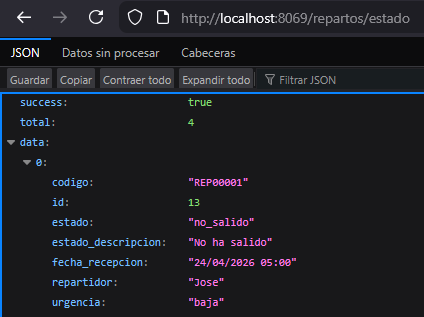
\includegraphics[width=0.8\textwidth]{img32.png}
    \end{figure}
Test desde elemento de prueba, aparece con codigo generico debido a que es una prueba anterior:
    \begin{figure}[H]
    \centering
    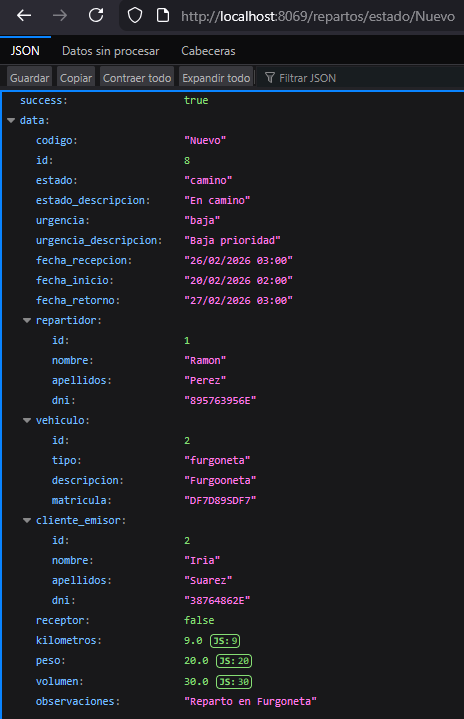
\includegraphics[width=0.8\textwidth]{img31.png}
    \end{figure}

El codigo lo genero mediante una api dentro de reparto. py: 
    \begin{lstlisting}[frame=single,breaklines=true]
@api.model
    def create(self, vals):
        if vals.get('codigo', 'Nuevo') == 'Nuevo':
            vals['codigo'] = self.env['ir.sequence'].next_by_code('reparto.reparto') or 'Nuevo'
        return super(Reparto, self).create(vals)
    \end{lstlisting}








\section{Security}
Aqui muestro el archivo de seguridad con los permisos basicos para cada modelo, simplemente doy acceso total como dice el ejercicio:
    \begin{lstlisting}[frame=single,breaklines=true]
    id,name,model_id:id,group_id:id,perm_read,perm_write,perm_create,perm_unlink
    access_reparto_empleado,access_reparto_empleado,model_reparto_empleado,base.group_user,1,1,1,1
    access_reparto_vehiculo,access_reparto_vehiculo,model_reparto_vehiculo,base.group_user,1,1,1,1
    access_reparto_cliente,access_reparto_cliente,model_reparto_cliente,base.group_user,1,1,1,1
    access_reparto_reparto,access_reparto_reparto,model_reparto_reparto,base.group_user,1,1,1,1
    \end{lstlisting}


\section{Casos de uso:}
En este apartado mostraré capturas de pantalla de cada uno de los casos de uso pedidos en el enunciado,
 mostrando el error que se produce al no cumplir la restriccion.
    \subsection{Reparto empleado sin carnet adecuado:}
    \begin{figure}[H]
    \centering
    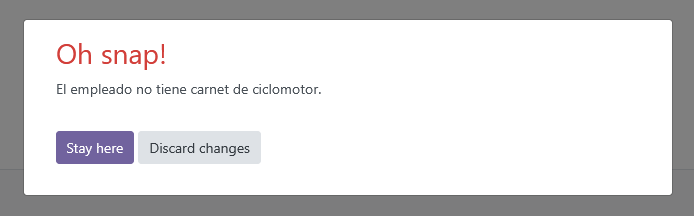
\includegraphics[width=0.8\textwidth]{img10.png}
    \end{figure}
        \begin{figure}[H]
    \centering
    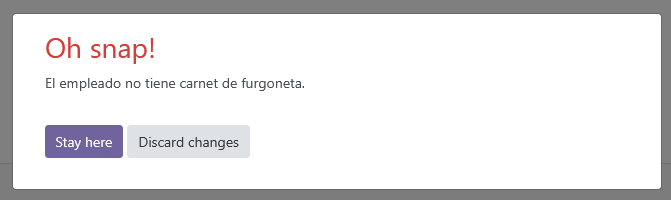
\includegraphics[width=0.8\textwidth]{img12.png}
    \end{figure}
    \subsection{Reparto empleado con carnet adecuado:}
    Permite crearla correctamente sin mostrar ningun error:
    \begin{figure}[H]
    \centering
    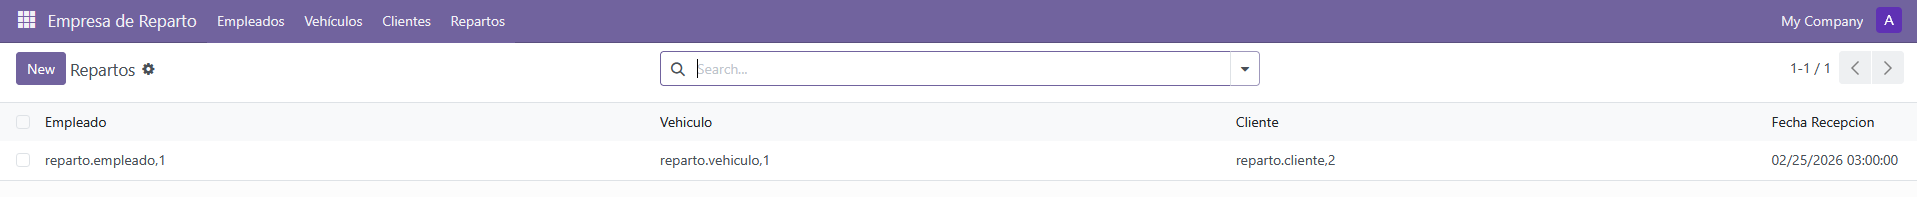
\includegraphics[width=0.8\textwidth]{img11.png}
    \end{figure}


    \subsection{Reparto con vehiculo ocupado:}
    \begin{figure}[H]
    \centering
    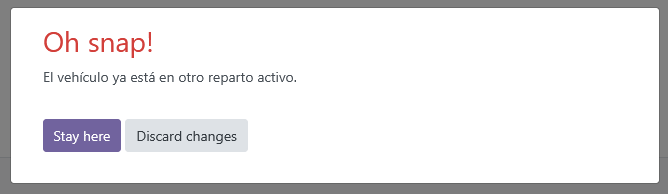
\includegraphics[width=0.8\textwidth]{img16.png}
    \end{figure}

    \subsection{Reparto con empleado ya activo:}
    \begin{figure}[H]
    \centering
    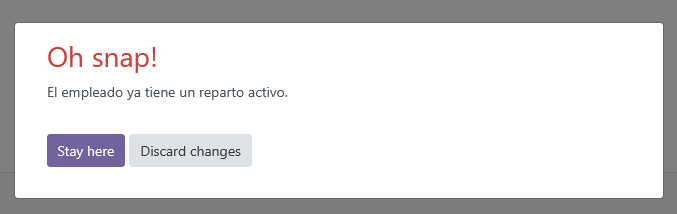
\includegraphics[width=0.8\textwidth]{img15.png}
    \end{figure}

    \subsection{Reparto de mas de 10km en bicicleta:}
    \begin{figure}[H]
    \centering
    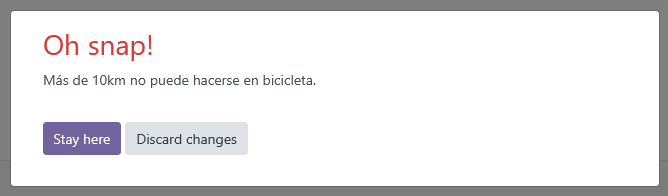
\includegraphics[width=0.8\textwidth]{img13.png}
    \end{figure}
    \subsection{Reparto de menos de 1km en furgoneta:}
    \begin{figure}[H]
    \centering
    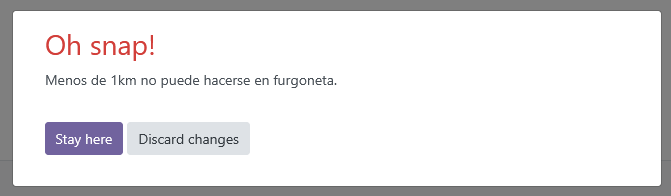
\includegraphics[width=0.8\textwidth]{img14.png}
    \end{figure}
Con este tenemos el ejercicio completo con las restricciones adecuadas, el wizard y el informe. Me encontre con numerosos porblemas los cuales
me hicieron perder horas, principalmente debido a como esta diseñado odoo, desde la lentitud para realizar cada prueba a los errores genericos
que normalmente no indican el problema real.
\end{document}

